\section{The Document Influence Model}
\label{section:model}

In this section we will develop a probabilistic model that captures
how past articles exhibit varying influence on future articles.  The
hypothesis is that an article's influence on the future is
corroborated by how the language of its field changes subsequent to
its publication.  In the model, the influence of each article is
encoded as a hidden variable; the posterior distribution of these
variables (given the text of documents) reveals the influential articles
of the collection.

\subsection*{Past approaches}
A number of algorithms link the text of documents to citation counts.
This work often models the information in citations by predicting them
or modeling them with
topics~\citep{nallapati:2008,chang:2009,dietz:2007,Cohn01themissing} or
other semantic tools \citep{mcnee:2002,ibanez:2009}.  Other work in
this area uses the text of documents along with citations to summarize
documents \citep{qazvinian:2008} or to propose new bibliometrics:
\cite{mann:2006} use topic models and citations to map topics over
time and define several new bibliometric measurements such as topic
Impact Factor, topical diffusion, and topic longevity.

Some work in this area uses the link structure of citation networks to
extract higher level structure. \cite{borner:2003}, for
example, have used author and citation networks to understand the
evolution of ideas in the history of science.

\subsection*{Dynamic Topics}
\begin{figure}
  \centering
  \begin{tabular}{cc}
    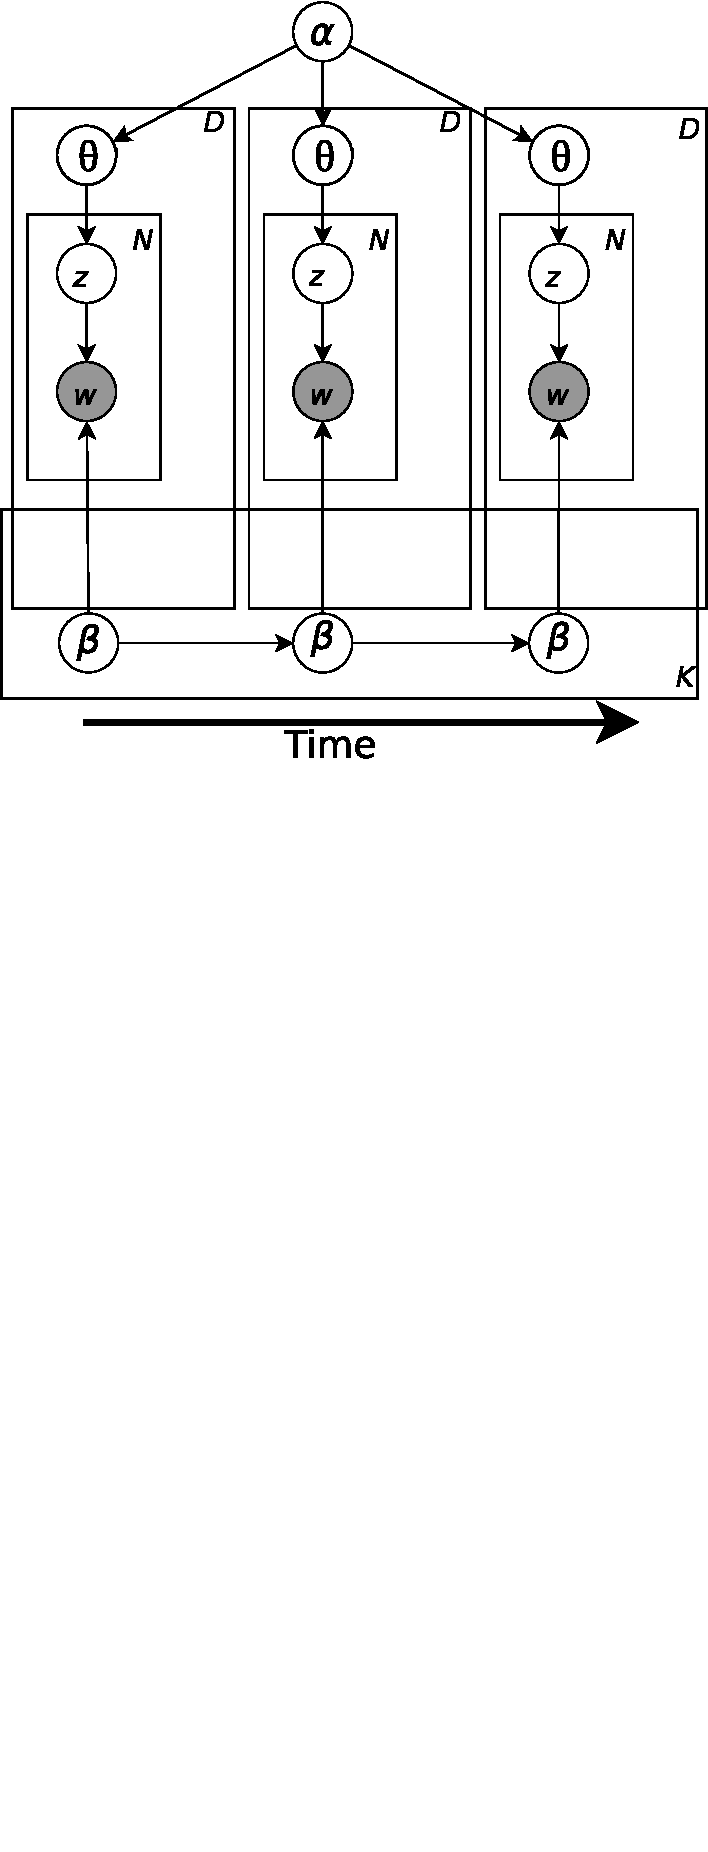
\includegraphics[width=0.3\textwidth,bb=50 500 350 800]{chapter_influence/figures/dtm_gm.pdf} &
    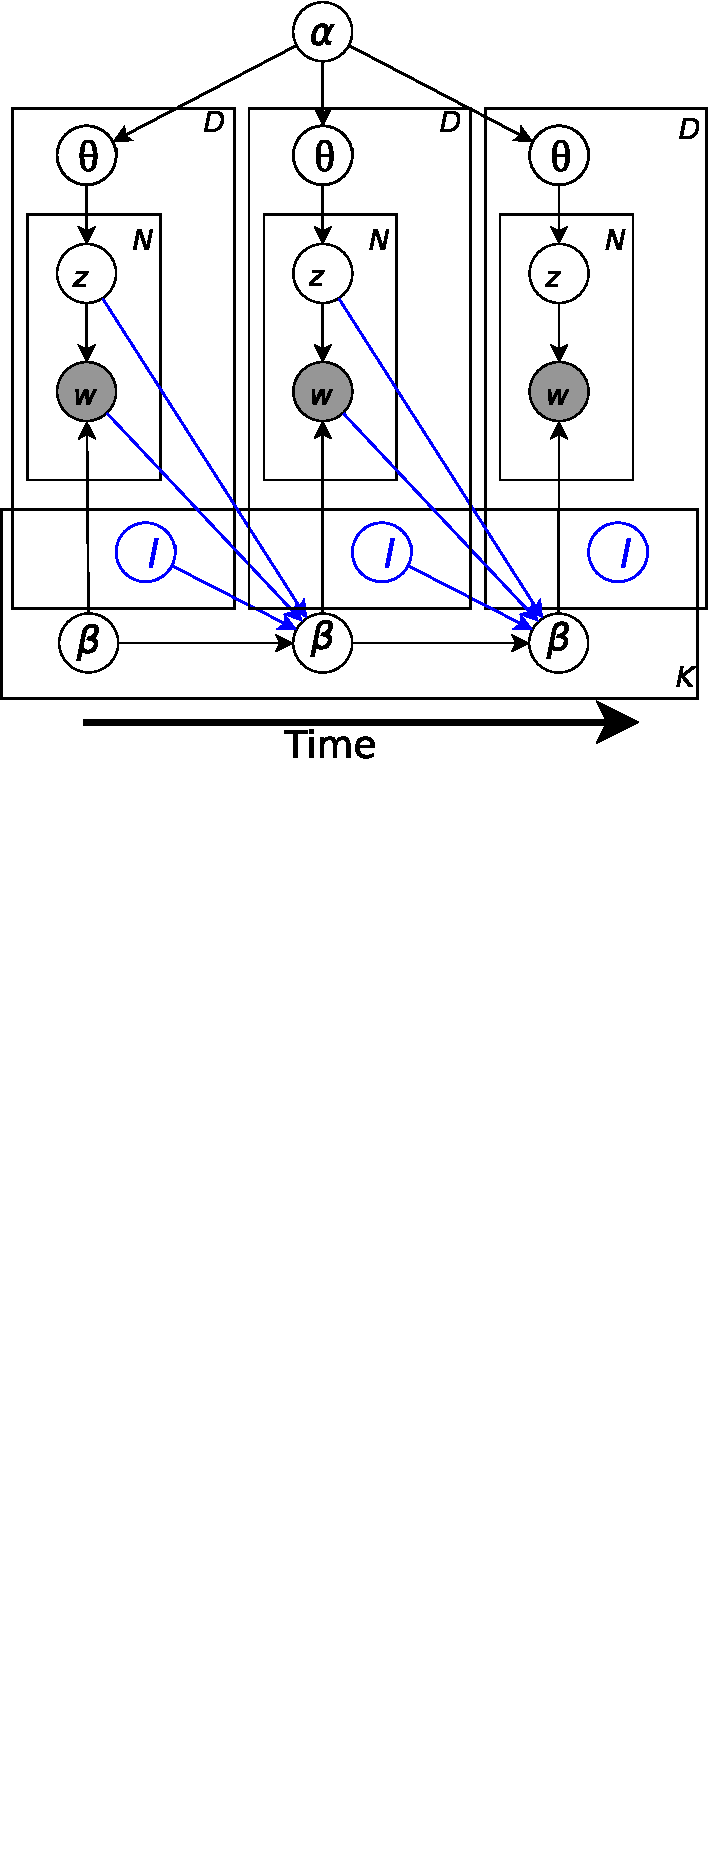
\includegraphics[width=0.3\textwidth,bb=-50 500 250 800]{chapter_influence/figures/docinf_gm.pdf} \\
    (a) & (b) \\
  \end{tabular}
 \label{fig:doc_influence_model}
  \caption{\label{fig:gm} The Dynamic Topic Model (a) and the the Document Influence Model (b).}
\end{figure}

Our model is based on the dynamic topic model (DTM)~\citep{blei:2006},
a model of sequential corpora that allows language statistics to drift
over time.  Probabilistic topic models such as LDA (introduced in the
last chapter) usually assume that the underlying distribution over
words is fixed \citep{blei:2003,deerwester:1990,hofmann:1999}. The DTM
introduced a Markov chain of term distributions to capture
probabilities that drift over the course of the collection.  The idea
is simple: topics drift in discrete steps over time.  At each
``epoch'', some number of documents are generated based on topics \emph{at that epoch}.

\paragraph{Drifting Topics.} We can formalize these assumptions in a
statistical model as in \cite{blei:2006}.  First let
$V$ be the number of words in a vocabulary and consider the natural
parameters $\beta_t$ of a term distribution at time $t$, where the
probability of a word $w$ is given by the softmax transformation of
the unconstrained vector,
\begin{equation}
  \label{eq:softmax}
  p(w \g \beta_{t}) \propto \exp(\beta_{t,w}).
\end{equation}
The corresponding distribution over terms, i.e., the ``topic,'' is a
point on the vocabulary simplex.  In the logistic normal Markov chain,
this distribution drifts with the stationary Markov process
\begin{equation}
  \label{eq:logistic-normal}
  \beta_{t+1} \g \beta_t \sim \mathcal{N}(\beta_{t}, \sigma^2 I),
\end{equation}
where $\sigma^2$ is the transition variance. 
% In the simplest DTM, a
% single distribution over words drifts according to
% \myeq{logistic-normal}.

\paragraph{Documents generated at time $t$.} Now consider a corpus
broken up into discrete epochs $t \in \{ 1, \ldots, T \}$, with $D_t$
articles at each time $t$.  Let $\W_{t,1:D}$ denote the articles as
vectors of word counts, where row $\w_{t,d}$ of $\W_{t, 1:D}$
represents the word counts in article $d$.

At each epoch $t$, the documents of these articles are drawn independently
using the topics described by \myeq{softmax}.  More formally, documents
are generated according to the generative model
\begin{enumerate}
\item For time $t=1, \ldots, T$:
  \begin{enumerate}
  \item For topics $k=1, \ldots, K$:
    \begin{enumerate}
    \item Draw topics $\beta_{k,t} \g \beta_{k,t-1} \sim \mathcal{N}(\beta_{k,t}, \sigma^2 I)$
    \end{enumerate}
  \item For document $d=1, \ldots, D_t$:
    \begin{enumerate}
    \item Draw topic mixture $\theta_d \sim \mbox{Dir}(\alpha, \ldots, \alpha)$.
    \item For term $n=1, \ldots, N$:
      \begin{enumerate}
      \item Draw topic indicator $z_n \sim \mbox{Mult}(\theta_d)$.
      \item Draw word $w_n$ according to \myeq{softmax}.
      \end{enumerate}
    \end{enumerate}
  \end{enumerate}
\end{enumerate}

We illustrate the graphical model for in \myfig{doc_influence_model} (a). With this
model in hand and a collection of documents, one can then estimate the
positions of these topics by computing the posterior distribution of
the sequence of topics $\beta_{1:T}$ conditioned on the observed
documents.  This summarizes the corpus as a smooth trajectory of word
frequencies.

\subsection*{The Document Influence Model}
We now turn to the original problem: certain ideas are influential in
the progression of a field, and we aim to discover what these ideas
are (as doing so will allow us to find those documents that are
influential).  The text of documents will provide a window into these
underlying patterns.

In our model, each article is assigned a normally distributed
\textit{influence score} $\ell_d$, which is a scalar value that
describes the influence that article $d$ has on the topic.  The higher
the influence, the more the words of the article affect how the topic
drifts.

This is encoded in the time series model.  The more influential a
document is, the more its words ``nudge'' the topic's natural
parameters at the next time step,
\begin{equation}
  \begin{split}
    \label{eq:logistic-normal-influence}
    \beta_{t+1} \g & \beta_t, (w, \ell)_{t,1:D} \sim
    \mathcal{N}\left(
      \beta_{t} +
      \exp(-\beta_t) \sum_d w_{d,t} \ell_{t,d},
      \sigma^2 I
    \right).
  \end{split}
\end{equation}
The words of an article with a high influence will have a higher
expected probability in the next epoch; the words of an article
with zero influence will not affect the next epoch.

% smg: Do you think the reader will understand the role of this term?
% The $\exp(-\beta_t)$ term makes influence meaningful in the space of
% natural parameters.

We call this model the \textit{document influence model}
(DIM). Conditioned on a corpus, the posterior distribution of the
topic and influence scores gives a trajectory of term frequencies and
a retrospective estimate of the influence of each article.  An article
whose words can help explain the way the word frequencies change will
have a high posterior influence score.  We will show in \mysec{results}
that this estimate of influence is meaningful.

\paragraph{Multiple topics.}  Corpora typically contain multiple
persistent themes.  Accordingly, the full dynamic topic model contains
multiple topics, each associated with a time series of distributions.
Conditioned on the topics, articles at each time are modeled
with latent Dirichlet allocation (LDA).  Each article exhibits the
topics with different random proportions $\theta_d$; each word of each
article is drawn by choosing a topic assignment from those proportions
$z_{d,n}$, and choosing a word from the corresponding topic
~\citep{blei:2003}.

Modeling multiple topics is important to the influence model because
an article might have different impact in the different fields that it
discusses.  For example, an article about computational genomics may
be very important to biology but less important to computer science.
We want to discern its influence on each of these topics separately.

As with the DTM, we posit $K$ topic trajectories, and each document of
each time point is modeled with LDA.  For each document, we now
associate an influence score $\ell_{d,k}$ for each topic $k$.  Each of
the $K$ topics drifts according to an adapted version of
\myeq{logistic-normal}, where we restrict attention to the influence
score for that topic and to the words of each document that were
assigned to it,
\begin{equation}
  \begin{split}
    \label{eq:logistic-normal-influence-topics}
    \beta_{k,t+1} & \g \beta_{k,t}, (w, \ell, z)_{t,1:D} \sim
    \mathcal{N}\left(
      \beta_{k,t} +
      \exp(-\beta_{k,t}) \sum_{d} \ell_{d,k} \sum_n w_{d,n} z_{d,n,k},
      \sigma^2 I
    \right).
  \end{split}
\end{equation}
Here, $z_{d,n,k}$ is the indicator that the $n$th word in document $d$
is assigned to topic $k$ and we have dropped the index $t$ on $z$ and
$w$.  The graphical model is illustrated \myfig{gm} (b).

Although we presented our model in this section with influence
spanning one year, we also adapted it to accomodate an ``influence
envelope'', where an article's influence spans $W$ years.  This
provides a more realistic model of influence \citep{porter:2005}, but
it complicates the inference algorithm and may not be necessary, as we
note in section~\ref{sec:results}.

% dmb: do we name the model anywhere as the DIM?
% smg: this is noted earlier (I think you added it in your rev.).

To use this model, we analyze a corpus through posterior inference.
This reveals a set of $K$ changing topics and influence scores for
each article and each topic.  The posterior provides a thematic window
into the corpus and can help identify which articles most contributed
to the development of its themes.

\subsection*{Work with similar goals}

It is worth pointing out two pieces of recent research which have similar
goals. \cite{leskovec:2009} describe a framework for tracking the
spread of memes, or ideas, in document collections, and investigate
the direction in which ideas tend to percolate.
\cite{shaparenko:2007} describe a measure of influence by modeling
documents as unigram mixtures of earlier documents and use a
likelihood ratio test to predict citations between documents. In
contrast to this work, the DIM uses dynamic topics to explicitly model
the change in \emph{topic} language.  Further, we do not attempt to
model links between documents, as in \cite{shaparenko:2007}.  % citet
